\section{Introduction}
The Asure ecosystem consists of the Asure Network, Asure Blockchain, the Asure Platform, and third-party applications. 

\begin{figure}[H]
    \centering
    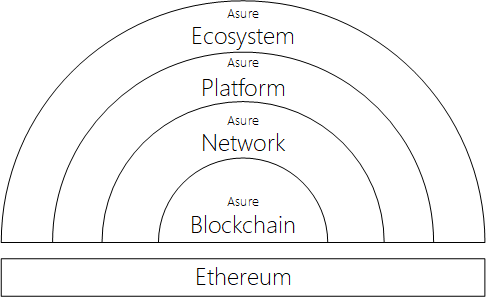
\includegraphics[width=4.0in]{img/ecosystem.png}
    \caption{Asure ecosystem}
    \label{fig:asure_ecosystem}
\end{figure}

The Asure network is a scalable blockchain network for decentralized social security systems. It lays the foundation for 10 billion people to have access to social security systems and achieves a great social impact where it is needed the most. \cite{worldometers} 

As the technological base that ensures optimal performance regarding the transaction throughput while maintaining the decentralized character of the network it guarantees the required level of transparency and cost-efficiency within the system. It is implemented as many Plasma side-chains that are connected to the Asure Blockchain as well as the Ethereum blockchain or any other EVM compatible blockchain. Each side-chain is operated by several independent node providers who need to stake ASR tokens to reach consensus between them and therefore within the network. By staking ASR tokens, node providers can earn additional tokens by offering their computing power. There will be a side-chain for each social security system within the Asure network.

The Asure Blockchain contains the Asure root-chain and connected side-chains. Root-chain offers advantages in the area of security as well as interchain communication. All running Asure Blockchain nodes represent the Asure Network. The Asure Platform connects the backend infrastructure to applications which can be used by end-users or programming interfaces for developers to build applications on top of the Asure platform. 


\subsection{Social security systems}
Social security is an insurance system in which the insured risks (such as illness, maternity, need for long-term care, accidents at work, work-related illness, unemployment, reduced earning capacity, old age and death) are covered jointly by all insured persons. Social security systems absorb many life risks, prevent extreme hardship and thus creates a social balance. 

People who do not have access to social security systems are at risk of falling into poverty if they are struck by a stroke of fate such as illness, crop failure or disability. They may then have to liquidate savings, sell livestock and other means of production and send their children to work instead of the school in order to finance daily expenses. \cite{erd}

People who enjoy basic social security are more willing to invest in education and physical capital, which entail additional risks, but also the prospect of income improvements. Empirical studies suggest that the existence of social security systems, especially in the informal sector, strengthens the propensity to invest and thus promotes economic growth precisely where this best contributes to poverty reduction. \cite{hcms}

It exists a broad spectrum of social security systems and they all vary in their concrete implementation. We define the functionality of the most common social security systems for the purpose of this paper as follows:

\subsubsection*{Pension}
A pension system consists of a number of contributors and pensioners. The contributors pay monthly premiums which get redistributed to the current pensioners. In return, the contributors have the right to receive their pension after a certain period of time, based on the time and amount of paid premiums. In some systems, the premiums get paid by the company on behalf of the contributor which would mean a massive reduction of transactions needed.
Pension payouts usually happen on a fixed date and all pensioners get paid at the same time. This makes it an ideal use case for mass payout transactions.

\subsubsection*{Healthcare}
The parties in healthcare are diverse - there are insured people who pay a premium there are doctors, hospitals, pharmacies and other service providers who issue invoices. These can be offset against the system or via the insured person who submits the invoices to the system and gets the costs reimbursed. Here there are different possibilities how you can realize the processing in batches, the insured can submit the accumulated invoices at the end of the year or the doctors, hospitals, pharmacies and other service providers can also submit their collective invoices in batches.

\subsubsection*{Unemployment}
Unemployment insurance is the protection against loss of work. Participants having a job pay a premium where in case of loss of work the time is bridged by the contributors to find a job again.

\subsubsection*{Social Care Insurance}

The Social Care Insurance, Long-term Care Insurance or Nursing Care Insurance  is a compulsory insurance to cover the risk of becoming dependent on long-term care. Social care insurance benefits are granted on the basis of "levels of need for long-term care". In the case of professional outpatient or (partly) inpatient care, the costs are covered up to a certain maximum amount (incl. nursing aids, measures to improve the living environment as well as voluntary nursing benefits). The compulsory Social Care Insurance is therefore not a full insurance. In order to achieve full coverage, it is necessary to take out a private supplementary nursing care insurance. In case of need, the insured person is entitled to assistance with nursing care as a needs-oriented supplementary social benefit.

\subsubsection*{Child And Youth Support}
In Germany, Child And Youth Support covers all services and tasks of public and independent institutions for the benefit of young people and their families. Child and youth welfare is not a direct pillar of social insurance, but is mainly provided by independent institutions, which work closely with the authorities. It is mainly financed by taxpayers' money. 

\subsubsection*{Invalidity insurance / Accident Insurance}
The purpose of statutory accident insurance is to prevent accidents at work, occupational diseases and work-related health risks and to restore the health and professional performance of the insured persons "by all appropriate means" after the occurrence of these insured events.

\subsection{Blockchain}
A blockchain is a decentralized database that holds a constantly growing list of transaction records. The database is extended chronologically linear, similar to a chain to which new elements are constantly added at the bottom (hence the term "blockchain"). If a block is complete, the next one is created. Each block contains a checksum of the previous block. Satoshi Nakamoto's development of Bitcoin in 2009 is one of the blockchain implementations which shows the potential for the technology for the finance transactions. \cite{bitcoin}

The disruptive potential of blockchain becomes increasingly apparent. After the invention of the Ethereum blockchain and Ethereum Virtual Machine (EVM), the world was given the tools necessary to build working decentralized autonomous organizations (DAO). In such a system, multiple authorities control different components and no single authority is fully trusted by all others. \cite{cammarden} The Blockchain technology is a perfect match to operate social security autonomously and decentralized.